\subsection{Obecná rovnice roviny}
\label{subsec:General_plane_equation}

V předchozí části jsme rovinu popisovali pomocí jednoho jejího bodu,
dvou směrových vektorů a dvou parametrů. Změnou parametrů jsme vytvářeli
jednotlivé body roviny. Parametrické vyjádření nám tedy říká,
\emph{jak body roviny získávat}.

Rovinu však můžeme popsat také jedinou rovnicí o třech proměnných $x$,
$y$ a $z$, kterou splňují právě souřadnice bodů ležících v této rovině.
Takový zápis umožňuje například rychle ověřit, zda daný bod v rovině leží,
nebo snadno porovnávat směry různých rovin. Tento způsob popisu nazýváme
\textbf{obecnou rovnicí roviny}.

Základní roli při jejím odvození bude hrát vektor, který je k rovině kolmý.

\subsubsection{Normálový vektor roviny}
\label{subsubsec:Normal_vector_plane}

Při parametrickém vyjádření roviny jsme její směry určovali pomocí dvou
navzájem nerovnoběžných směrových vektorů. Nyní budeme místo nich pracovat
s vektorem, který je kolmý ke všem směrům ležícím v rovině.

\begin{definition}
    \label{def:Normal_vector_plane}
    \textbf{Normálovým vektorem roviny} $\alpha$ nazýváme každý nenulový
    vektor $\vec{n}$, který je kolmý k této rovině.
\end{definition}

Je-li rovina $\alpha$ určena dvěma směrovými vektory $\vec{u}$ a
$\vec{v}$ a je-li $\vec{n}$ jejím normálovým vektorem, potom platí
\begin{equation}
    \vec{n}\cdot\vec{u}=0
    \qquad\text{a}\qquad
    \vec{n}\cdot\vec{v}=0.
    \label{eq:Normal_vector_plane_orthogonality}
\end{equation}

Normálový vektor je tedy kolmý k oběma nezávislým směrům roviny. Protože
každý další směrový vektor roviny vznikne jako lineární kombinace
$\vec{u}$ a $\vec{v}$, je normálový vektor kolmý také ke každému dalšímu
vektoru ležícímu v rovině.

Známe-li dva navzájem nerovnoběžné směrové vektory roviny, můžeme
normálový vektor určit pomocí jejich vektorového součinu:
\begin{equation}
    \vec{n}=\vec{u}\times\vec{v}.
    \label{eq:Normal_vector_plane_cross_product}
\end{equation}

Vektorový součin je kolmý k oběma násobeným vektorům, a proto je kolmý
také k rovině, kterou tyto vektory určují.

\begin{figure}[H]
    \centering
    \begin{tikzpicture}[scale=0.9]

        % Rovina
        \coordinate (P1) at (-1.3,0.1,0.2);
        \coordinate (P2) at (4.3,1.2,0.8);
        \coordinate (P3) at (5.0,3.7,2.8);
        \coordinate (P4) at (-0.6,2.6,2.2);

        \fill[gray!18] (P1) -- (P2) -- (P3) -- (P4) -- cycle;
        \draw[thin] (P1) -- (P2) -- (P3) -- (P4) -- cycle;

        % Osy - kladná část
        \draw[->] (0,0,0) -- (5.2,0,0) node[right] {$x$};
        \draw[->] (0,0,0) -- (0,4.6,0) node[above] {$y$};
        \draw[->] (0,0,0) -- (0,0,4.2) node[below left] {$z$};

        % Osy - záporná část
        \draw[->, dashed] (0,0,0) -- (-2.2,0,0);
        \draw[->, dashed] (0,0,0) -- (0,-2.2,0);
        \draw[->, dashed] (0,0,0) -- (0,0,-2.7);

        \node[above left] at (0,0,0) {$O$};

        % Bod a vektory
        \coordinate (A) at (1.4,1.3,1.3);
        \coordinate (U) at (3.6,1.75,1.5);
        \coordinate (V) at (2.0,2.65,2.3);
        \coordinate (N) at (1.4,2.0,3.7);

        \draw[vector] (A) -- (U)
            node[midway, sloped, above] {$\vec{u}$};
        \draw[vector] (A) -- (V)
            node[midway, sloped, above] {$\vec{v}$};
        \draw[vector] (A) -- (N)
            node[midway, right] {$\vec{n}$};

        % Naznačení pravého úhlu
        \draw
            (1.62,1.43,1.42)
            -- (1.58,1.61,1.63)
            -- (1.36,1.51,1.57);

        \fill (A) circle (2pt) node[below left] {$A$};
        \node at (4.25,3.1,2.55) {$\alpha$};

    \end{tikzpicture}
    \caption{Směrové vektory $\vec{u}$ a $\vec{v}$ leží v rovině
    $\alpha$, zatímco normálový vektor $\vec{n}$ je k rovině kolmý.}
    \label{fig:Normal_vector_plane}
\end{figure}

Stejně jako směrové vektory ani normálový vektor není určen jednoznačně.
Je-li $\vec{n}$ normálovým vektorem roviny, potom je jejím normálovým
vektorem také každý jeho nenulový reálný násobek
\[
    k\vec{n},
    \qquad
    k\in\mathbb{R}\setminus\{0\}.
\]
Všechny tyto vektory jsou navzájem rovnoběžné a jsou kolmé k téže rovině.

\subsubsection{Odvození obecné rovnice roviny}
\label{subsubsec:Derivation_general_plane_equation}

Uvažujme rovinu $\alpha$, která prochází bodem
\[
    A[x_A;y_A;z_A]
\]
a má normálový vektor
\[
    \vec{n}=(a;b;c),
\]
kde alespoň jedna ze souřadnic $a$, $b$, $c$ je nenulová. Dále zvolme
libovolný bod prostoru
\[
    X[x;y;z].
\]

Vektor směřující z bodu $A$ do bodu $X$ má souřadnice
\[
    \overrightarrow{AX}
    =(x-x_A;y-y_A;z-z_A).
\]

Bod $X$ leží v rovině $\alpha$ právě tehdy, když vektor
$\overrightarrow{AX}$ leží ve směru této roviny. Proto musí být kolmý
k normálovému vektoru $\vec{n}$. Pomocí skalárního součinu tuto podmínku
zapíšeme jako
\begin{equation}
    \vec{n}\cdot\overrightarrow{AX}=0.
    \label{eq:Point_normal_condition_plane}
\end{equation}

Po dosazení souřadnic obou vektorů dostáváme
\begin{align*}
    (a;b;c)\cdot(x-x_A;y-y_A;z-z_A)&=0,\\
    a(x-x_A)+b(y-y_A)+c(z-z_A)&=0.
\end{align*}

Rovnice
\begin{equation}
    a(x-x_A)+b(y-y_A)+c(z-z_A)=0
    \label{eq:Point_normal_plane_equation}
\end{equation}
popisuje rovinu, která prochází bodem $A[x_A;y_A;z_A]$ a má normálový
vektor $\vec{n}=(a;b;c)$. Tento zápis můžeme nazývat
\textbf{bodově-normálovým tvarem rovnice roviny}.

\begin{figure}[H]
    \centering
    \begin{tikzpicture}[scale=0.9]

        % Rovina
        \coordinate (P1) at (-1.3,0.1,0.2);
        \coordinate (P2) at (4.3,1.2,0.8);
        \coordinate (P3) at (5.0,3.7,2.8);
        \coordinate (P4) at (-0.6,2.6,2.2);

        \fill[gray!18] (P1) -- (P2) -- (P3) -- (P4) -- cycle;
        \draw[thin] (P1) -- (P2) -- (P3) -- (P4) -- cycle;

        % Osy - kladná část
        \draw[->] (0,0,0) -- (5.2,0,0) node[right] {$x$};
        \draw[->] (0,0,0) -- (0,4.6,0) node[above] {$y$};
        \draw[->] (0,0,0) -- (0,0,4.2) node[below left] {$z$};

        % Osy - záporná část
        \draw[->, dashed] (0,0,0) -- (-2.2,0,0);
        \draw[->, dashed] (0,0,0) -- (0,-2.2,0);
        \draw[->, dashed] (0,0,0) -- (0,0,-2.7);

        \node[above left] at (0,0,0) {$O$};

        % Body
        \coordinate (A) at (1.2,1.2,1.2);
        \coordinate (X) at (3.7,2.5,2.1);
        \coordinate (Y) at (3.1,2.1,3.5);
        \coordinate (N) at (1.2,1.9,3.6);

        \fill (A) circle (2pt) node[below left] {$A$};
        \fill (X) circle (2pt) node[below right] {$X$};
        \fill (Y) circle (2pt) node[above right] {$Y$};

        % Vektory
        \draw[vector] (A) -- (X)
            node[midway, sloped, below] {$\overrightarrow{AX}$};
        \draw[vector] (A) -- (N)
            node[midway, right] {$\vec{n}$};
        \draw[vector, dashed] (A) -- (Y)
            node[midway, sloped, above] {$\overrightarrow{AY}$};

        % Bod Y mimo rovinu
        \draw[dashed] (Y) -- (2.8,1.85,2.6);

        \node at (4.25,3.1,2.55) {$\alpha$};

    \end{tikzpicture}
    \caption{Bod $X$ leží v rovině $\alpha$, protože vektor
    $\overrightarrow{AX}$ je kolmý k normálovému vektoru $\vec{n}$.
    U bodu $Y$, který v rovině neleží, tato kolmost neplatí.}
    \label{fig:General_plane_derivation}
\end{figure}

Roznásobením rovnice~\eqref{eq:Point_normal_plane_equation} získáme
\begin{align*}
    a(x-x_A)+b(y-y_A)+c(z-z_A)&=0,\\
    ax-ax_A+by-by_A+cz-cz_A&=0,\\
    ax+by+cz-(ax_A+by_A+cz_A)&=0.
\end{align*}

Bod $A$ i normálový vektor $\vec{n}$ jsou pevně zvolené, a proto je
výraz
\[
    -(ax_A+by_A+cz_A)
\]
konstantou. Označíme-li tuto konstantu písmenem $d$, dostáváme rovnici
\[
    ax+by+cz+d=0.
\]

\begin{definition}
    \label{def:General_plane_equation}
    \textbf{Obecnou rovnicí roviny} v prostoru nazýváme rovnici tvaru
    \begin{equation}
        ax+by+cz+d=0,
        \label{eq:General_plane_equation}
    \end{equation}
    kde
    \[
        a,b,c,d\in\mathbb{R}
        \qquad\text{a}\qquad
        (a;b;c)\neq(0;0;0).
    \]

    Rovina $\alpha$ je množinou všech bodů $X[x;y;z]$, jejichž souřadnice
    tuto rovnici splňují, tedy
    \[
        X[x;y;z]\in\alpha
        \quad\Longleftrightarrow\quad
        ax+by+cz+d=0.
    \]
\end{definition}

Koeficienty $a$, $b$, $c$ jsou souřadnicemi normálového vektoru roviny:
\begin{equation}
    \vec{n}_{\alpha}=(a;b;c).
    \label{eq:Normal_vector_from_general_plane}
\end{equation}

Koeficient $d$ ovlivňuje polohu roviny v prostoru. Při pevných
koeficientech $a$, $b$, $c$ mají všechny rovnice
\[
    ax+by+cz+d=0
\]
stejný normálový vektor, a popisují proto navzájem rovnoběžné roviny nebo
tutéž rovinu.

Podmínka $(a;b;c)\neq(0;0;0)$ je nezbytná. Kdyby současně platilo
$a=b=c=0$, rovnice by se zredukovala na vztah
\[
    d=0.
\]
Pro $d=0$ by ji splňoval každý bod prostoru, zatímco pro $d\neq0$ by ji
nesplňoval žádný bod. Ani v jednom případě by tedy rovnice nepopisovala
rovinu.

\subsubsection{Rovina určená bodem a normálovým vektorem}
\label{subsubsec:Plane_point_normal_vector}

Známe-li jeden bod roviny a její normálový vektor, můžeme obecnou rovnici
sestavit přímo z bodově-normálového tvaru.

\begin{example}
    \label{exa:General_plane_point_normal}
    Určete obecnou rovnici roviny $\alpha$, která prochází bodem
    \[
        A[-2;3;2]
    \]
    a má normálový vektor
    \[
        \vec{n}=(1;-1;4).
    \]

    Použijeme bodově-normálový tvar
    \[
        a(x-x_A)+b(y-y_A)+c(z-z_A)=0.
    \]
    Po dosazení bodu a normálového vektoru dostáváme
    \begin{align*}
        1(x-(-2))-1(y-3)+4(z-2)&=0,\\
        x+2-y+3+4z-8&=0,\\
        x-y+4z-3&=0.
    \end{align*}

    Obecná rovnice roviny je
    \[
        \alpha:\quad x-y+4z-3=0.
    \]
\end{example}

Stejný výsledek můžeme získat také tak, že nejprve zapíšeme rovnici
s neznámým koeficientem $d$:
\[
    x-y+4z+d=0.
\]
Dosadíme souřadnice bodu $A[-2;3;2]$:
\[
    -2-3+4\cdot2+d=0,
\]
odkud
\[
    d=-3.
\]

Oba postupy jsou rovnocenné. První přímo využívá bodově-normálový tvar,
druhý nejprve sestaví tvar obecné rovnice z normálového vektoru a následně
určí koeficient $d$ dosazením bodu roviny.

\begin{remark}
    Je-li znám bod $A[x_A;y_A;z_A]$ a normálový vektor
    $\vec{n}=(a;b;c)$, můžeme koeficient $d$ určit přímo ze vztahu
    \[
        d=-(ax_A+by_A+cz_A).
    \]
\end{remark}

\subsubsection{Čtení informací z obecné rovnice}
\label{subsubsec:Reading_general_plane_equation}

Z obecné rovnice roviny můžeme okamžitě vyčíst její normálový vektor.
Například rovina
\[
    \beta:\quad 2x-3y+z+5=0
\]
má normálový vektor
\[
    \vec{n}_{\beta}=(2;-3;1).
\]

Každý nenulový násobek tohoto vektoru je také normálovým vektorem roviny,
například
\[
    (-4;6;-2)
    \qquad\text{nebo}\qquad
    (6;-9;3).
\]

Naopak nelze z obecné rovnice přímo vyčíst jeden konkrétní směrový vektor
roviny. Směrových vektorů ležících v rovině je nekonečně mnoho. Každý
z nich však musí být kolmý k normálovému vektoru. Vektor
\[
    \vec{u}=(u_x;u_y;u_z)
\]
je tedy směrovým vektorem roviny $\beta$ právě tehdy, když platí
\[
    (2;-3;1)\cdot(u_x;u_y;u_z)=0,
\]
tedy
\[
    2u_x-3u_y+u_z=0.
\]

Například vektory
\[
    \vec{u}=(3;2;0)
    \qquad\text{a}\qquad
    \vec{v}=(-1;0;2)
\]
jsou směrovými vektory roviny $\beta$, protože
\[
    2\cdot3-3\cdot2+0=0
\]
a
\[
    2\cdot(-1)-3\cdot0+2=0.
\]

\subsubsection{Příslušnost bodu k rovině}
\label{subsubsec:Point_membership_general_plane}

Chceme-li rozhodnout, zda bod $P[x_P;y_P;z_P]$ leží v rovině
\[
    \alpha:\quad ax+by+cz+d=0,
\]
dosadíme jeho souřadnice za proměnné $x$, $y$ a $z$.

Jestliže po dosazení dostaneme pravdivou rovnost
\[
    ax_P+by_P+cz_P+d=0,
\]
bod v rovině leží. Pokud levá strana vyjde nenulová, bod v rovině neleží.

\begin{example}
    \label{exa:Point_membership_general_plane}
    Rozhodněte, zda body
    \[
        P[4;-2;4]
        \qquad\text{a}\qquad
        Q[3;-1;3]
    \]
    leží v rovině
    \[
        \alpha:\quad x-5y-3z-2=0.
    \]

    Pro bod $P[4;-2;4]$ dostáváme
    \[
        4-5(-2)-3\cdot4-2
        =4+10-12-2
        =0.
    \]
    Bod $P$ tedy rovnici splňuje, a proto
    \[
        P\in\alpha.
    \]

    Pro bod $Q[3;-1;3]$ dostáváme
    \[
        3-5(-1)-3\cdot3-2
        =3+5-9-2
        =-3\neq0.
    \]
    Bod $Q$ rovnici nesplňuje, a proto
    \[
        Q\notin\alpha.
    \]
\end{example}

\subsubsection{Nejednoznačnost obecné rovnice roviny}
\label{subsubsec:Nonuniqueness_general_plane_equation}

Obecná rovnice roviny není určena jednoznačně. Vynásobíme-li všechny
koeficienty rovnice stejným nenulovým reálným číslem, množina jejích
řešení se nezmění.

Například rovnice
\[
    x-5y-3z-2=0
\]
a
\[
    -2x+10y+6z+4=0
\]
popisují tutéž rovinu. Druhá rovnice vznikla vynásobením první rovnice
číslem $-2$.

Obecně rovnice
\[
    ax+by+cz+d=0
\]
a
\[
    kax+kby+kcz+kd=0,
    \qquad
    k\in\mathbb{R}\setminus\{0\},
\]
popisují tutéž rovinu.

\begin{remark}
    Jsou-li všechny koeficienty obecné rovnice celočíselné a mají
    společného dělitele, můžeme rovnici tímto dělitelem vydělit. Získáme
    jednodušší rovnici téže roviny.
\end{remark}

\subsubsection{Rovina procházející počátkem soustavy souřadnic}
\label{subsubsec:Plane_through_origin}

Rovina
\[
    \alpha:\quad ax+by+cz+d=0
\]
prochází počátkem soustavy souřadnic $O[0;0;0]$ právě tehdy, když bod
$O$ splňuje její rovnici. Po dosazení dostáváme
\[
    a\cdot0+b\cdot0+c\cdot0+d=0,
\]
tedy
\[
    d=0.
\]

\begin{remark}
    Rovina prochází počátkem soustavy souřadnic právě tehdy, když její
    obecná rovnice nemá absolutní člen:
    \[
        ax+by+cz=0.
    \]
\end{remark}

Například rovina
\[
    2x-y+3z=0
\]
počátkem prochází, zatímco rovina
\[
    2x-y+3z-4=0
\]
počátkem neprochází.

\subsubsection{Význam nulových koeficientů}
\label{subsubsec:Zero_coefficients_general_plane}

Nulový koeficient u některé proměnné znamená, že rovnice na příslušné
souřadnici nezávisí.

Uvažujme například rovinu
\[
    \alpha:\quad by+cz+d=0,
\]
ve které je koeficient $a$ roven nule. Jestliže bod $A[x_A;y_A;z_A]$
v této rovině leží, potom v ní leží také každý bod
\[
    X[x;y_A;z_A],
    \qquad
    x\in\mathbb{R},
\]
protože změna $x$-ové souřadnice hodnotu levé strany rovnice nijak
neovlivní.

V rovině tedy můžeme procházet ve směru vektoru
\[
    (1;0;0),
\]
který je směrovým vektorem osy $x$. Rovina je proto rovnoběžná s osou
$x$.

Obdobně platí:

\begin{itemize}
    \item jestliže $a=0$, je rovina rovnoběžná s osou $x$;
    \item jestliže $b=0$, je rovina rovnoběžná s osou $y$;
    \item jestliže $c=0$, je rovina rovnoběžná s osou $z$.
\end{itemize}

Tuto skutečnost můžeme vysvětlit také pomocí normálového vektoru. Je-li
$a=0$, má normálový vektor tvar
\[
    \vec{n}=(0;b;c).
\]
Pro směrový vektor osy $x$
\[
    \vec{e}_x=(1;0;0)
\]
platí
\[
    \vec{n}\cdot\vec{e}_x=0,
\]
a proto je směr osy $x$ rovnoběžný s rovinou.

Zvláštními případy jsou souřadnicové roviny:
\[
    xy:\quad z=0,
\]
\[
    xz:\quad y=0,
\]
\[
    yz:\quad x=0.
\]

Rovnice
\[
    x=k
\]
popisuje rovinu rovnoběžnou se souřadnicovou rovinou $yz$. Podobně
rovnice
\[
    y=k
\]
popisuje rovinu rovnoběžnou s rovinou $xz$ a rovnice
\[
    z=k
\]
rovinu rovnoběžnou s rovinou $xy$.

\subsubsection{Rovina rovnoběžná s danou rovinou}
\label{subsubsec:Parallel_plane_through_point}

Rovnoběžné roviny mají rovnoběžné normálové vektory. Chceme-li proto
sestavit rovnici roviny rovnoběžné s danou rovinou, můžeme použít stejný
normálový vektor a dopočítat pouze nový koeficient $d$.

\begin{example}
    \label{exa:Parallel_plane_through_point}
    Určete obecnou rovnici roviny $\beta$, která je rovnoběžná s rovinou
    \[
        \alpha:\quad x-y+4z-3=0
    \]
    a prochází bodem
    \[
        S[1;3;-2].
    \]

    Normálový vektor roviny $\alpha$ je
    \[
        \vec{n}_{\alpha}=(1;-1;4).
    \]
    Rovina $\beta$ může mít stejný normálový vektor, a proto její rovnici
    zapíšeme ve tvaru
    \[
        x-y+4z+d=0.
    \]

    Dosadíme bod $S[1;3;-2]$:
    \[
        1-3+4(-2)+d=0.
    \]
    Odtud
    \[
        d=10.
    \]

    Hledaná rovina má rovnici
    \[
        \beta:\quad x-y+4z+10=0.
    \]
\end{example}

Roviny $\alpha$ a $\beta$ mají stejné koeficienty u proměnných $x$, $y$,
$z$, ale různé absolutní členy. Mají proto stejný normálový směr, ale
nejsou totožné.

\subsubsection{Rovina určená třemi body}
\label{subsubsec:General_plane_three_points}

Jsou-li dány tři body $A$, $B$ a $C$, které neleží na jedné přímce,
můžeme nejprve určit dva směrové vektory roviny:
\[
    \vec{u}=\overrightarrow{AB},
    \qquad
    \vec{v}=\overrightarrow{AC}.
\]
Normálový vektor roviny potom získáme jejich vektorovým součinem:
\[
    \vec{n}=\vec{u}\times\vec{v}.
\]

Nakonec použijeme jeden ze zadaných bodů a sestavíme obecnou rovnici.

\begin{example}
    \label{exa:General_plane_three_points}
    Určete obecnou rovnici roviny $\alpha$, která prochází body
    \[
        A[2;1;3],
        \qquad
        B[3;3;1],
        \qquad
        C[1;2;5].
    \]

    Nejprve určíme dva směrové vektory roviny:
    \[
        \vec{u}
        =\overrightarrow{AB}
        =(3-2;3-1;1-3)
        =(1;2;-2)
    \]
    a
    \[
        \vec{v}
        =\overrightarrow{AC}
        =(1-2;2-1;5-3)
        =(-1;1;2).
    \]

    Normálový vektor získáme vektorovým součinem:
    \[
        \vec{n}
        =\vec{u}\times\vec{v}
        =(1;2;-2)\times(-1;1;2)
        =(6;0;3).
    \]
    Všechny souřadnice můžeme vydělit číslem $3$, a jako normálový vektor
    proto zvolíme
    \[
        \vec{n}=(2;0;1).
    \]

    Obecná rovnice má tvar
    \[
        2x+z+d=0.
    \]
    Dosadíme například bod $A[2;1;3]$:
    \[
        2\cdot2+3+d=0,
    \]
    odkud
    \[
        d=-7.
    \]

    Hledaná rovina má rovnici
    \[
        \alpha:\quad 2x+z-7=0.
    \]

    Správnost ověříme dosazením zbývajících bodů:
    \[
        B[3;3;1]:
        \qquad
        2\cdot3+1-7=0,
    \]
    \[
        C[1;2;5]:
        \qquad
        2\cdot1+5-7=0.
    \]
    Všechny tři body rovnici splňují.
\end{example}

\begin{remark}
    Jestliže by vektorový součin
    $\overrightarrow{AB}\times\overrightarrow{AC}$ vyšel nulový, byly by
    vektory $\overrightarrow{AB}$ a $\overrightarrow{AC}$ rovnoběžné.
    Body $A$, $B$ a $C$ by potom ležely na jedné přímce a neurčovaly by
    jedinou rovinu.
\end{remark}

\subsubsection{Převod parametrického vyjádření na obecnou rovnici}
\label{subsubsec:Parametric_to_general_plane}

Je-li rovina zadána parametricky, můžeme z jejího zápisu vyčíst jeden bod
a dva směrové vektory. Jejich vektorovým součinem získáme normálový vektor
a následně sestavíme obecnou rovnici.

\begin{example}
    \label{exa:Parametric_to_general_plane}
    Převeďte parametrické vyjádření roviny
    \[
        \begin{aligned}
            \alpha: x&=1+2s+t,\\
            y&=-2+s-t,\\
            z&=3-s+2t; s,t\in\mathbb{R}
        \end{aligned}
    \]
    na obecnou rovnici.

    Z parametrického vyjádření vyčteme bod
    \[
        A[1;-2;3]
    \]
    a směrové vektory
    \[
        \vec{u}=(2;1;-1),
        \qquad
        \vec{v}=(1;-1;2).
    \]

    Normálový vektor získáme vektorovým součinem:
    \[
        \vec{n}
        =\vec{u}\times\vec{v}
        =(2;1;-1)\times(1;-1;2)
        =(1;-5;-3).
    \]

    Obecná rovnice má tvar
    \[
        x-5y-3z+d=0.
    \]
    Dosadíme bod $A[1;-2;3]$:
    \[
        1-5(-2)-3\cdot3+d=0.
    \]
    Odtud
    \[
        d=-2.
    \]

    Obecná rovnice roviny je
    \[
        \alpha:\quad x-5y-3z-2=0.
    \]
\end{example}

Správnost převodu můžeme zkontrolovat tím, že do obecné rovnice dosadíme
parametrické výrazy:
\begin{align*}
    x-5y-3z-2
    &=(1+2s+t)-5(-2+s-t)-3(3-s+2t)-2\\
    &=1+2s+t+10-5s+5t-9+3s-6t-2\\
    &=0.
\end{align*}
Výsledek je nulový pro libovolné hodnoty parametrů $s$ a $t$, a proto
každý bod parametricky zadané roviny splňuje získanou obecnou rovnici.

\subsubsection{Převod obecné rovnice na parametrické vyjádření}
\label{subsubsec:General_to_parametric_plane}

Při převodu obecné rovnice na parametrické vyjádření máme jednu rovnici
se třemi proměnnými. Dvě proměnné proto můžeme zvolit jako nezávislé
parametry a třetí pomocí nich vyjádřit.

Kterou proměnnou budeme dopočítávat, závisí na tom, který z koeficientů
$a$, $b$, $c$ je nenulový.

Je-li například $a\neq0$, můžeme v rovnici
\[
    ax+by+cz+d=0
\]
zvolit
\[
    y=s,
    \qquad
    z=t,
    \qquad
    s,t\in\mathbb{R}.
\]
Potom
\[
    ax=-bs-ct-d
\]
a
\[
    x=-\frac{d}{a}-\frac{b}{a}s-\frac{c}{a}t.
\]

Parametrické vyjádření roviny má tedy tvar
\[
    \begin{aligned}
        \alpha: x&=-\frac{d}{a}-\frac{b}{a}s-\frac{c}{a}t,\\
        y&=s,\\
        z&=t; s,t\in\mathbb{R}.
    \end{aligned}
\]

\begin{example}
    \label{exa:General_to_parametric_plane}
    Převeďte obecnou rovnici
    \[
        \alpha:\quad x-5y-3z-2=0
    \]
    na parametrické vyjádření.

    Zvolíme
    \[
        y=s,
        \qquad
        z=t,
        \qquad
        s,t\in\mathbb{R}.
    \]
    Z obecné rovnice vyjádříme souřadnici $x$:
    \begin{align*}
        x-5s-3t-2&=0,\\
        x&=2+5s+3t.
    \end{align*}

    Parametrické vyjádření je
    \[
        \begin{aligned}
            \alpha: x&=2+5s+3t,\\
            y&=s,\\
            z&=t; s,t\in\mathbb{R}.
        \end{aligned}
    \]

    Z tohoto zápisu můžeme vyčíst bod
    \[
        B[2;0;0]
    \]
    a směrové vektory
    \[
        \vec{u}=(5;1;0),
        \qquad
        \vec{v}=(3;0;1).
    \]
    Oba jsou kolmé k normálovému vektoru
    \[
        \vec{n}=(1;-5;-3),
    \]
    protože
    \[
        (1;-5;-3)\cdot(5;1;0)=5-5=0
    \]
    a
    \[
        (1;-5;-3)\cdot(3;0;1)=3-3=0.
    \]
\end{example}

Při jiném výběru parametrů můžeme získat jiný bod i jiné směrové vektory,
ale výsledná rovina zůstane stejná.

\subsubsection{Rovina kolmá k přímce}
\label{subsubsec:Plane_perpendicular_to_line}

Je-li rovina kolmá k přímce, je směrový vektor této přímky rovnoběžný
s normálovým vektorem roviny. Směrový vektor přímky proto můžeme při
sestavování obecné rovnice použít jako normálový vektor roviny.

\begin{example}
    \label{exa:Plane_perpendicular_to_line}
    Určete obecnou rovnici roviny $\alpha$, která je kolmá k přímce
    \[
        \begin{aligned}
            p: x&=1+2t,\\
            y&=-2+t,\\
            z&=3-t; t\in\mathbb{R}
        \end{aligned}
    \]
    a prochází bodem
    \[
        A[1;2;3].
    \]

    Směrový vektor přímky je
    \[
        \vec{u}_p=(2;1;-1).
    \]
    Protože je rovina $\alpha$ k přímce kolmá, můžeme tento vektor použít
    jako normálový vektor roviny:
    \[
        \vec{n}_{\alpha}=(2;1;-1).
    \]

    Obecná rovnice má tvar
    \[
        2x+y-z+d=0.
    \]
    Dosadíme bod $A[1;2;3]$:
    \[
        2\cdot1+2-3+d=0,
    \]
    odkud
    \[
        d=-1.
    \]

    Hledaná rovina má rovnici
    \[
        \alpha:\quad 2x+y-z-1=0.
    \]
\end{example}

\subsubsection{Průsečíky roviny se souřadnicovými osami}
\label{subsubsec:Plane_axis_intercepts}

Průsečík roviny se souřadnicovou osou musí současně ležet v rovině i na
dané ose.

Na ose $x$ mají body tvar
\[
    P[p;0;0].
\]
Dosazením do obecné rovnice
\[
    ax+by+cz+d=0
\]
dostáváme
\[
    ap+d=0.
\]
Je-li $a\neq0$, potom
\[
    p=-\frac{d}{a}.
\]

Podobně pro průsečíky s osami $y$ a $z$ dostáváme
\[
    q=-\frac{d}{b},
    \qquad
    r=-\frac{d}{c},
\]
pokud jsou příslušné koeficienty nenulové.

Rovina se tedy při $a,b,c\neq0$ protíná se souřadnicovými osami v bodech
\[
    P\left[-\frac{d}{a};0;0\right],
\]
\[
    Q\left[0;-\frac{d}{b};0\right],
\]
\[
    R\left[0;0;-\frac{d}{c}\right].
\]

\subsubsection{Úsekový tvar rovnice roviny}
\label{subsubsec:Intercept_form_plane}

Jestliže se rovina protíná se všemi třemi souřadnicovými osami v bodech
\[
    P[p;0;0],
    \qquad
    Q[0;q;0],
    \qquad
    R[0;0;r],
\]
kde
\[
    p,q,r\neq0,
\]
můžeme její rovnici zapsat v úsekovém tvaru
\begin{equation}
    \frac{x}{p}+\frac{y}{q}+\frac{z}{r}=1.
    \label{eq:Intercept_form_plane}
\end{equation}

Čísla $p$, $q$, $r$ jsou orientované úseky, které rovina vytíná na
souřadnicových osách. Mohou být kladná i záporná.

\begin{example}
    \label{exa:Intercept_form_plane}
    Určete úsekový i obecný tvar rovnice roviny, která protíná
    souřadnicové osy v bodech
    \[
        P[6;0;0],
        \qquad
        Q[0;3;0],
        \qquad
        R[0;0;4].
    \]

    Z průsečíků přímo sestavíme úsekový tvar:
    \[
        \frac{x}{6}+\frac{y}{3}+\frac{z}{4}=1.
    \]

    Rovnici vynásobíme nejmenším společným násobkem jmenovatelů, tedy
    číslem $12$:
    \[
        2x+4y+3z=12.
    \]
    Obecná rovnice roviny je
    \[
        2x+4y+3z-12=0.
    \]
\end{example}

\begin{figure}[H]
    \centering
    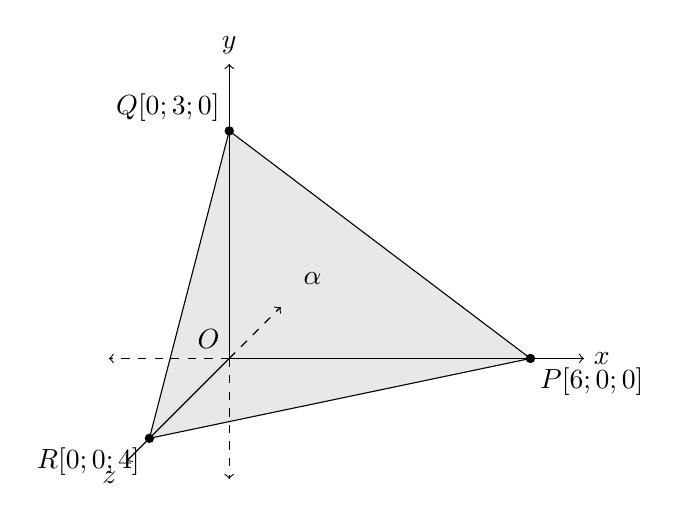
\begin{tikzpicture}[scale=0.85]

        % Průsečíky s osami
        \coordinate (P) at (4.5,0,0);
        \coordinate (Q) at (0,3.4,0);
        \coordinate (R) at (0,0,3.1);

        % Část roviny určená průsečíky
        \fill[gray!18] (P) -- (Q) -- (R) -- cycle;
        \draw[thin] (P) -- (Q) -- (R) -- cycle;

        % Osy - kladná část
        \draw[->] (0,0,0) -- (5.3,0,0) node[right] {$x$};
        \draw[->] (0,0,0) -- (0,4.4,0) node[above] {$y$};
        \draw[->] (0,0,0) -- (0,0,4.0) node[below left] {$z$};

        % Osy - záporná část
        \draw[->, dashed] (0,0,0) -- (-1.8,0,0);
        \draw[->, dashed] (0,0,0) -- (0,-1.8,0);
        \draw[->, dashed] (0,0,0) -- (0,0,-2.0);

        \node[above left] at (0,0,0) {$O$};

        % Body
        \fill (P) circle (2pt) node[below right] {$P[6;0;0]$};
        \fill (Q) circle (2pt) node[above left] {$Q[0;3;0]$};
        \fill (R) circle (2pt) node[below left] {$R[0;0;4]$};

        \node at (1.9,1.85,1.7) {$\alpha$};

    \end{tikzpicture}
    \caption{Rovina určená svými průsečíky se souřadnicovými osami.}
    \label{fig:Plane_intercept_form}
\end{figure}

Úsekový tvar nelze použít v každé situaci. Jestliže je některý
z koeficientů $a$, $b$, $c$ nulový, je rovina rovnoběžná s příslušnou
osou a nemá s ní jediný průsečík. Jestliže rovina prochází počátkem,
je některý z úseků nulový a ve jmenovateli úsekového tvaru by vznikla
nula.

\subsubsection{Shrnutí}
\label{subsubsec:General_plane_summary}

Obecná rovnice roviny má tvar
\[
    ax+by+cz+d=0,
\]
kde alespoň jeden z koeficientů $a$, $b$, $c$ je nenulový.

Z této rovnice můžeme vyčíst normálový vektor
\[
    \vec{n}=(a;b;c).
\]

Bod $P[x_P;y_P;z_P]$ leží v rovině právě tehdy, když po dosazení jeho
souřadnic platí
\[
    ax_P+by_P+cz_P+d=0.
\]

Obecnou rovnici můžeme sestavit zejména tehdy, když známe:

\begin{itemize}
    \item bod roviny a její normálový vektor;
    \item tři nekolineární body roviny;
    \item parametrické vyjádření roviny;
    \item rovinu, se kterou má být hledaná rovina rovnoběžná, a jeden bod;
    \item přímku, ke které má být hledaná rovina kolmá, a jeden bod.
\end{itemize}

Obecná rovnice je vhodná pro ověřování příslušnosti bodů a pro práci
s normálovým směrem roviny. V následujících částech ji využijeme při
zkoumání vzájemné polohy rovin a při určování vztahů mezi přímkami
a rovinami.
